\section{Concluding remarks}
The elegant drawings of blinks and blackboard framed links produced by BLINK are 
possible due the groundbreaking algorithm of R. Tamasia \cite{tamassia1987egg}.
Lauro could implement the drawings very fast because we had at hand the implementation of
network flow algorithms he had done for a project to solve {\em practical timetable (!) problems}.
This is an example of the unicity in Mathematics, advocated by L. Lovasz in his famous essay \cite{lovasz1998om}.
To get the drawings one has to apply three times the full strength of network flow theory.
The drawings BLINK presents are in an integer grid and 
deterministically minimize the number of $\pi/2$-bents in the blackboarded framed links.
In particular, it permit us to deal with the unavoidable curls which adjust the integer framings in
the best possible way: we do not care about them. 
The drawings for the companion blinks require a slight modification: it replaces each $p$-valent vertex $p>4$,
by a $p$-polygon inducing 3-valent ones. The final result is massaged a bit to
produce aesthetically pleasing and unambiguous drawings.

As of this writing, C. Hodgson sent me some puzzling 
information (computed with a stronger version of SnapPy) about the first pair of 
manifolds. These are induced by $T[71]$ and $T[79]$, forming the $HG8QI$-class $14_{24}^t$.
They are non-homeomorphic 3-manifolds as first shown by N. Dunfield.
They are homology $\mathbb{Z}$-spheres which have the same WRT-invariants 
(according to BLINK), and quoting Craig {\em ``the same volume (around 24.8) and the same lenght spectra (up to 12 decimals):
the (complex) length of the first geodesic of $T[71]$ is 
0.4749346632398791 + 0i  (of multiplicity 1) 
and that of $T[79]$ is 0.4749346632399361 + 0 i  (of multiplicity 1).''}

\noindent
Here are the Dirichlet domains:
\begin{center}
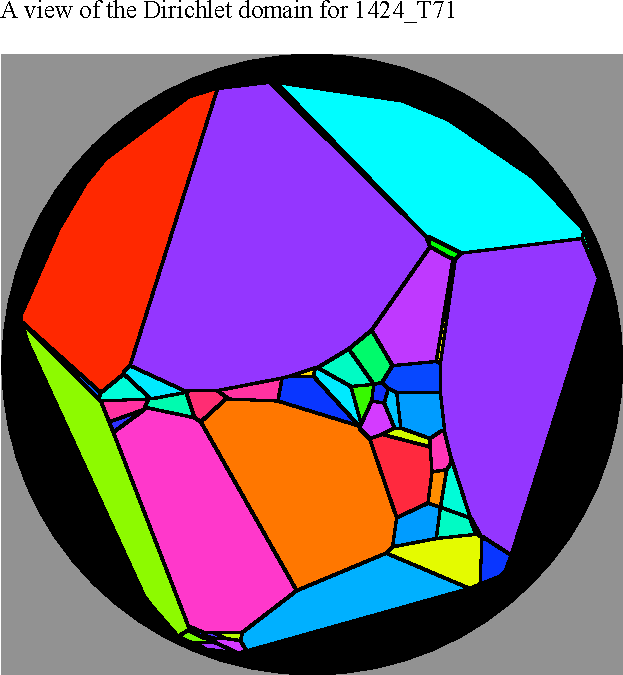
\includegraphics[width=7cm]{1.figs/DirDomT71.pdf}
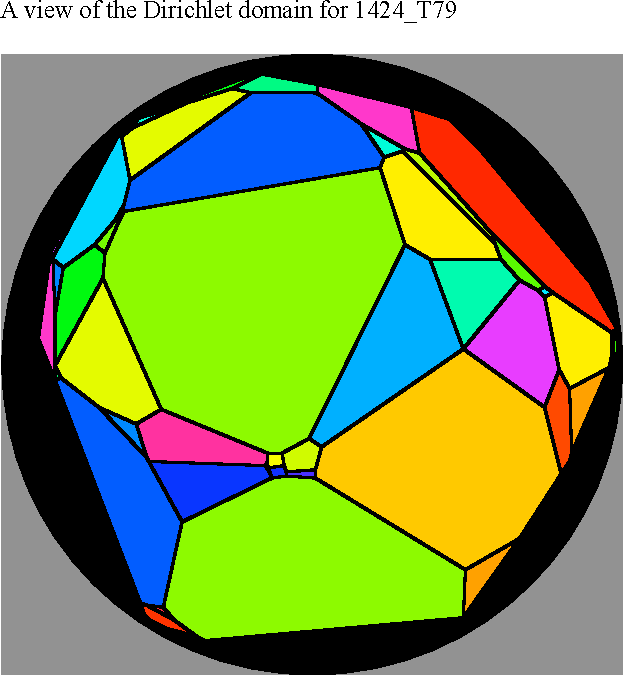
\includegraphics[width=7cm]{1.figs/DirDomT79.pdf}
\end{center}

\noindent
Craig found another proof that $T[71]$ and $T[79]$ are non-homemorphic:
{\em
``Now we can drill out the shortest geodesics using SnapPea to obtain
one-cusped manifolds (the manifold files are attached).
Then SnapPea's isometry checker (which uses the canonical cell decompositions) 
shows that these cusped manifolds are not isometric. Hence the original
closed manifolds are not homeomorphic.
This gives another proof that  $T[71]$ and $T[79]$ are distinct!''}

\noindent
{\bf A final challenge:} 
From the data I could get so far, if a closed orientable 3-manifold is hyperbolic, 
it seems that the WRT-invariants determine its volume. 
Prove it or disproved it.

%-----------------------------------
\bibliographystyle{plain}
%\bibliographystyle{is-alpha}
%\addcontentsline{toc}{bibliografia}{\MakeTextUppercase{Referências Bibliográficas}}
%\bibliography{d:/slsl\3.DadosSostenes.35.ArtigosLivros.bibtexGoogleScholar/bibtexIndex.bib} % bib file is slsl.bib
%\bibliography{~/home/ricardo/Dropbox/35.ArtigosLivros.bibtexGoogleScholar/bibtexIndex.bib}
\bibliography{bibtexIndex.bib}
%\bibliography{slsl}


\vspace{5mm}
\begin{center}
\hspace{7mm}
\begin{tabular}{l}
   S\'ostenes L. Lins\\
   Centro de Inform\'atica, UFPE \\
   Av. Jornalista Anibal Fernandes s/n\\
   Recife, PE 50740-560 \\
   Brazil\\
   sostenes@cin.ufpe.br
\end{tabular}
\end{center}
